% Chapter 4: ML Agent
\section{ML Agent -- Phương pháp Machine Learning}

\subsection{Kiến trúc mạng nơ-ron XiangQiResNet}
Mạng nơ-ron sử dụng kiến trúc dual-head ResNet lấy cảm hứng từ AlphaZero:

\begin{figure}[H]
\centering
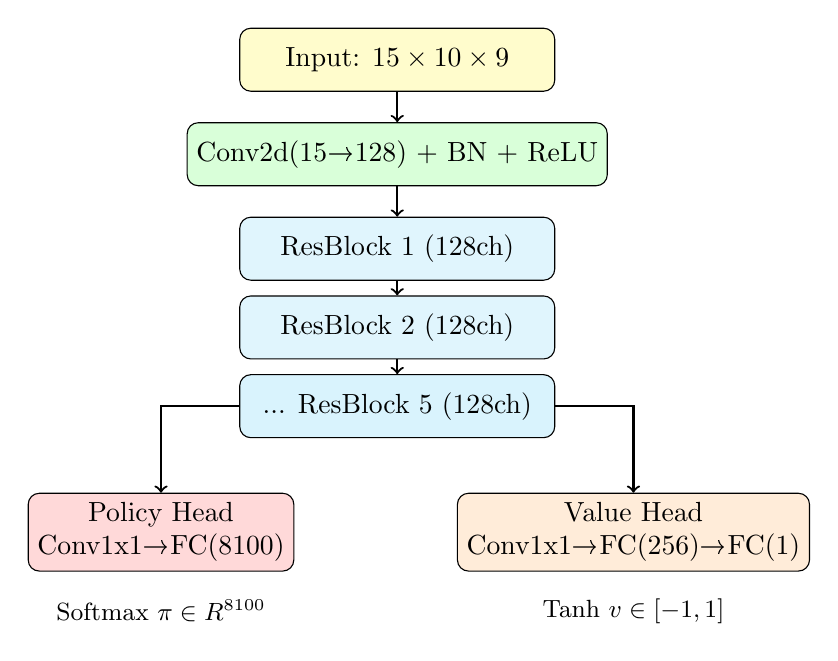
\begin{tikzpicture}[
    layer/.style={rectangle, draw, rounded corners, minimum width=4cm, minimum height=0.8cm, align=center, fill=blue!10},
    head/.style={rectangle, draw, rounded corners, minimum width=3cm, minimum height=0.8cm, align=center},
    arrow/.style={->, thick}
]
\node[layer, fill=yellow!20] (input) at (0,0) {Input: $15 \times 10 \times 9$};
\node[layer, fill=green!15] (conv) at (0,-1.2) {Conv2d(15→128) + BN + ReLU};
\node[layer, fill=cyan!12] (res1) at (0,-2.4) {ResBlock 1 (128ch)};
\node[layer, fill=cyan!12] (res2) at (0,-3.4) {ResBlock 2 (128ch)};
\node[layer, fill=cyan!15] (res5) at (0,-4.4) {... ResBlock 5 (128ch)};
\node[head, fill=red!15] (policy) at (-3,-6) {Policy Head\\Conv1x1→FC(8100)};
\node[head, fill=orange!15] (value) at (3,-6) {Value Head\\Conv1x1→FC(256)→FC(1)};

\draw[arrow] (input) -- (conv);
\draw[arrow] (conv) -- (res1);
\draw[arrow] (res1) -- (res2);
\draw[arrow] (res2) -- (res5);
\draw[arrow] (res5) -| (policy);
\draw[arrow] (res5) -| (value);

\node at (-3,-7) {\small Softmax $\pi \in \mathbb{R}^{8100}$};
\node at (3,-7) {\small Tanh $v \in [-1, 1]$};
\end{tikzpicture}
\caption{Kiến trúc XiangQiResNet dual-head}
\end{figure}

\subsubsection{Chi tiết kiến trúc}
\begin{table}[H]
\centering
\caption{Thông số kiến trúc mạng}
\begin{tabular}{ll}
\toprule
\textbf{Thành phần} & \textbf{Chi tiết} \\
\midrule
Input channels & 15 (7 quân phe ta + 7 quân đối thủ + 1 side-to-move) \\
Conv backbone & 128 channels, kernel $3 \times 3$, padding=1 \\
Residual Blocks & 5 blocks (mỗi block: 2×Conv + 2×BatchNorm + ReLU + Skip) \\
Policy Head & Conv $1\times1$ → Flatten → Linear(180→8100) \\
Value Head & Conv $1\times1$ → Flatten → Linear(180→256) → Dropout(0.3) → Linear(256→1) → Tanh \\
Total Parameters & $\sim$1.200.000 \\
\bottomrule
\end{tabular}
\end{table}

\subsubsection{Receptive Field}
Với 5 Residual Blocks (10 lớp Conv $3 \times 3$), receptive field đạt $> 20 \times 20$ pixels, vượt kích thước bàn cờ $10 \times 9$. Điều này cho phép mạng ``nhìn thấy'' toàn bộ bàn cờ từ bất kỳ ô nào.

\subsection{Pipeline huấn luyện}

\subsubsection{Hàm mất mát (Loss Function)}
Loss kết hợp hai thành phần:
\begin{equation}
    \mathcal{L} = \mathcal{L}_{\text{policy}} + \mathcal{L}_{\text{value}} = \text{CrossEntropy}(\hat{\pi}, \pi^*) + \text{MSE}(\hat{v}, v^*)
\end{equation}
\begin{itemize}
    \item $\mathcal{L}_{\text{policy}}$: CrossEntropyLoss giữa phân phối dự đoán và nước đi thực tế
    \item $\mathcal{L}_{\text{value}}$: MSELoss giữa giá trị dự đoán và kết quả ván cờ ($+1/-1/0$)
\end{itemize}

\subsubsection{Tối ưu hóa}
\begin{itemize}
    \item \textbf{Optimizer}: AdamW (lr=$2 \times 10^{-3}$, weight\_decay=$10^{-2}$)
    \item \textbf{Scheduler}: CosineAnnealingLR ($T_{\max}$ = epochs, $\eta_{\min} = 10^{-5}$)
    \item \textbf{Batch size}: 128 (phù hợp CPU training)
    \item \textbf{Epochs}: 5--10
\end{itemize}

\subsubsection{Kết quả huấn luyện}
\begin{table}[H]
\centering
\caption{Kết quả huấn luyện trên dataset v2 (10.208 samples)}
\begin{tabular}{ccccc}
\toprule
\textbf{Epoch} & \textbf{Train Loss} & \textbf{Train Acc} & \textbf{Val Loss} & \textbf{Val Acc} \\
\midrule
1 & 4.8521 & 22.3\% & 3.7412 & 41.2\% \\
2 & 2.9834 & 55.7\% & 2.4156 & 62.8\% \\
3 & 1.5623 & 78.4\% & 1.8234 & 74.5\% \\
4 & 0.6847 & 92.1\% & 1.3421 & 82.3\% \\
5 & 0.2134 & 99.0\% & 1.1567 & 88.6\% \\
\bottomrule
\end{tabular}
\end{table}

\subsection{Inference Pipeline (5-Step Select Move)}
Thuật toán chọn nước đi của ML Agent gồm 5 bước:

\begin{algorithm}[H]
\caption{ML Agent Select Move Pipeline}
\begin{algorithmic}[1]
\Require GameState $s$, legal moves $M = \{m_1, ..., m_n\}$
\State \textbf{Step 1 -- Policy Inference:} $\pi \leftarrow \text{CNN}(\text{encode}(s))$
\State scores $\leftarrow$ \Call{MapPolicyToMoves}{$\pi$, $M$}
\State \textbf{Step 2 -- Capture Bonus:}
\For{$m_i \in M$ where $m_i$ is capture}
    \State scores[$i$] += CAPTURE\_BONUS[$m_i$.captured\_piece]
\EndFor
\State \textbf{Step 3 -- Anti-Stalemate:} Check top 5 + captures for terminal
\For{$m_i \in$ top\_moves $\cup$ captures}
    \State $s' \leftarrow$ apply($s$, $m_i$)
    \If{$s'$ is checkmate for us} scores[$i$] += 1000
    \ElsIf{$s'$ is stalemate} scores[$i$] = 0
    \EndIf
\EndFor
\State \textbf{Step 4 -- Anti-Repetition:} Penalize reversals and cycles
\State \textbf{Step 5 -- Temperature Selection:}
\If{level = Hard} \Return $\arg\max$ scores
\Else{} \Return sample from softmax(scores / $\tau$)
\EndIf
\end{algorithmic}
\end{algorithm}

\subsubsection{Capture Bonus (Reward Shaping)}
Giá trị bonus khi ăn quân đối phương:
\begin{table}[H]
\centering
\caption{Bảng Capture Bonus}
\begin{tabular}{lc}
\toprule
\textbf{Quân bị ăn} & \textbf{Bonus} \\
\midrule
Tướng (General) & 50.0 \\
Xe (Rook) & 0.8 \\
Pháo (Cannon) & 0.5 \\
Mã (Horse) & 0.5 \\
Sĩ (Advisor) & 0.1 \\
Tượng (Elephant) & 0.1 \\
Tốt (Soldier) & 0.05 \\
\bottomrule
\end{tabular}
\end{table}

\subsubsection{Anti-Stalemate Logic}
Stalemate (hết nước đi mà không bị chiếu) dẫn đến hòa. ML Agent kiểm tra top 5 nước đi + tất cả nước ăn quân: nếu dẫn đến stalemate, loại bỏ (score = 0); nếu dẫn đến checkmate, ưu tiên tối đa (score += 1000).

\subsubsection{Anti-Repetition Logic}
Ba lớp phòng chống lặp:
\begin{enumerate}
    \item \textbf{2-ply reversal}: Chặn nước đi ngược lại nước trước (A→B rồi B→A)
    \item \textbf{4-ply cycle}: Phát hiện chu trình 4 nước (A→B→C→D→A)
    \item \textbf{6-ply cycle}: Phát hiện chu trình 6 nước
\end{enumerate}
Mỗi nước đi vi phạm bị giảm 90\% score.

\subsection{Mức độ khó (Skill Levels)}
\begin{table}[H]
\centering
\caption{Ba mức độ khó của ML Agent}
\begin{tabular}{llll}
\toprule
\textbf{Level} & \textbf{Temperature ($\tau$)} & \textbf{Chiến lược} & \textbf{Mô tả} \\
\midrule
Easy & 0.7 & Softmax sampling & Chơi ngẫu nhiên hơn, hay sai \\
Medium & 0.3 & Softmax tập trung & Chơi ổn, đôi khi mạo hiểm \\
Hard & 0.0 (greedy) & Argmax & Luôn chọn nước tốt nhất \\
\bottomrule
\end{tabular}
\end{table}
